\section{Genetic Algorithm}

\begin{frame}
    \frametitle{Curse of Dimentionality}
    \begin{itemize}
        \item As the variety of goods increase, the state space grows exponentially.
        \item Impossible to take all enumerations of classifiers into account when initializing. 
        \item Genetic algorithm will be considered.
    \end{itemize}
    
    \pause

    Four steps for adding and deleting incumbent classifiers:
    \begin{enumerate}
        \item Creation
        \item Diversification
        \item Specialization
        \item Generalization
    \end{enumerate}
\end{frame}

\begin{frame}
    \frametitle{Creation}

    \begin{block}{Activation}
        There are no classifier that matches the current state $z_{at}$, i.e., 
        $|\Me|=0$.
    \end{block}

    \begin{block}{Action}
        Assign random action to the current state $z_{at}$ and add it to the 
        collection of classifiers.
    \end{block}
\end{frame}


\begin{frame}[allowframebreaks]
    \frametitle{Diversification}
    
    \begin{block}{Activation}
        After the matched collection of classifiers $\Me$ are constructed.

        If for all $e \in \Me$ have the same action.
    \end{block}

    \begin{block}{Action}
        Assign opposite action to the current state $z_{at}$ and add it to the 
        collection of classifiers.
        
        Assign the strength of the winning classifier to that of the new one.
    \end{block}
    \framebreak

    There is also a deletion process
    \begin{block}{Deletion}
        Remove a "weak" classifier from the set of $\Me$. 
        The weakness is defined jointly with the strength $\Se$ and  winning counter $\tau_e^a(t)$ 
        
    \end{block}
\end{frame}

\begin{frame}
    \frametitle{Specialization}

    \begin{block}{Activation}
        After the winning bit has been determined. 
        Activation probability decreases over time.

        The winning classifier has some ambiguous position (\#).
    \end{block}

    \begin{block}{Action}
        Add a new classifier, which changes the \#s in the condition part of the current winning classifier
        with some probability.
        
        If the \# is changed, it changes to the correspond value of the state.
        
    \end{block}

    \begin{block}{Deletion}
        A weak rule is replaced by the new rule above.
    \end{block}

\end{frame}

\begin{frame}
    \frametitle{Generalization}
    \begin{block}{Activation}
        Called randomly after the above variation steps are conducted.

        The activation probability decreases over time.
    \end{block}

    \begin{block}{Initialization}
        Draw \emph{potential parents} and \emph{potential exterminants}. 
        The probability of drawing depends on some fitness criterion.
    \end{block}

\end{frame}

\begin{frame}
    \frametitle{Generalizarion - Mating}
    \begin{enumerate}
        \item Pick two parents to mate
        \item Pick two position in the classifier
        \item Pick to alter the \emph{inner} or \emph{outer} part of the slicing
        \item Inconsistent positions are replaced with ambiguity symbol \# 
    \end{enumerate}
        \begin{figure}
            \centering
            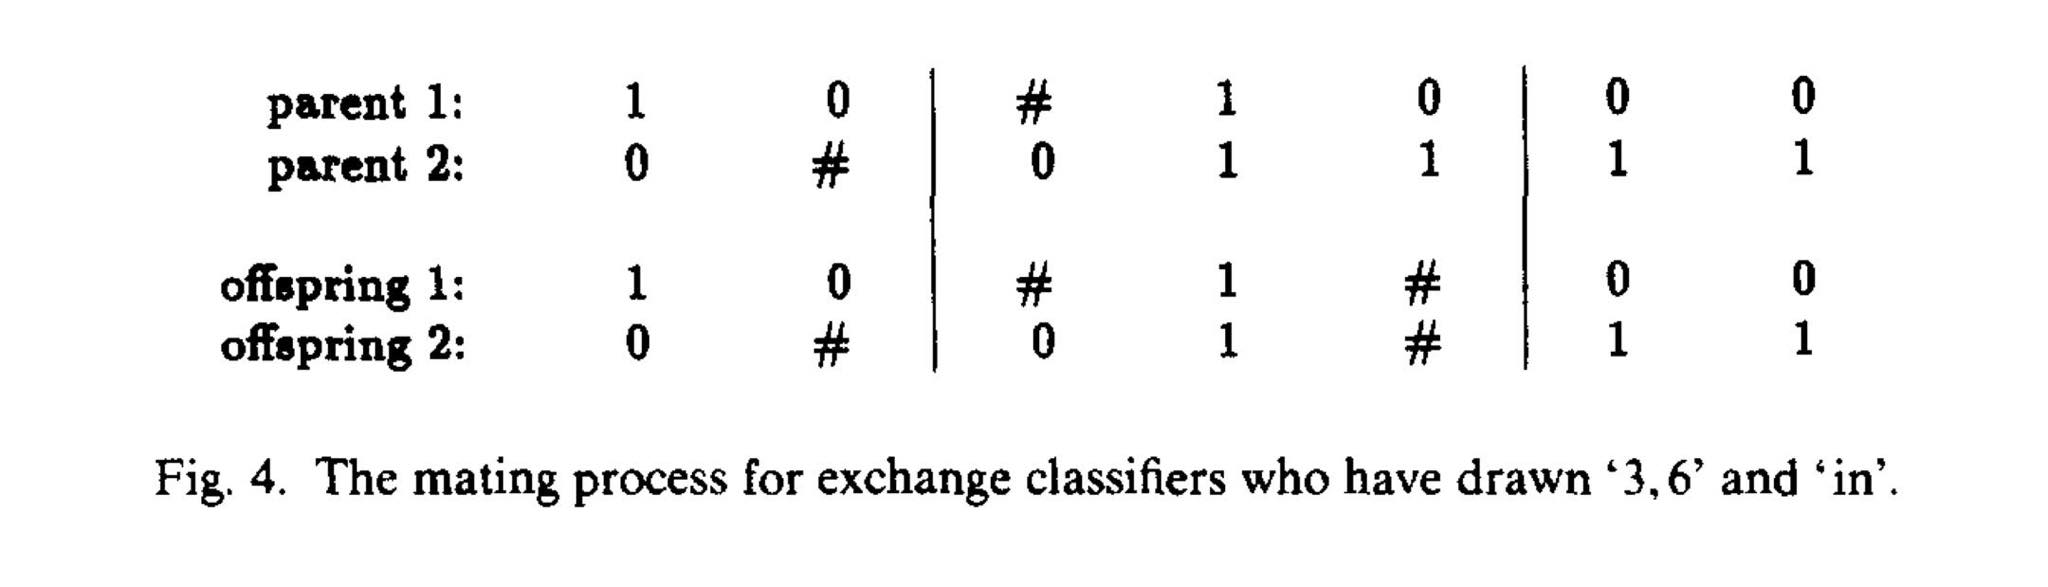
\includegraphics[width=\textwidth]{img/fig3_mating.jpg}
        \end{figure}
        \begin{enumerate}
            \item[5] Strength is set to be the average of its parents
        \end{enumerate}    

\end{frame}

\begin{frame}
    \frametitle{Generalization - Exterminating}

    Remove one of the random selected classifier from the potential exterminants set.
    
\end{frame}